\documentclass[10pt, a4paper]{article}
\usepackage[utf8]{inputenc}
\usepackage{amssymb}
\usepackage{pgf}
\usepackage{tikz}
\usetikzlibrary{arrows,automata}
\usetikzlibrary{graphs}
\usetikzlibrary{graphs.standard}
\usepackage{bsymb,b2latex}
\usepackage{algorithmic}
\usepackage{stmaryrd}

\newcommand{\BtoDA}[2]{
    \begin{minipage}[c]{.45\linewidth}
    #1
    \end{minipage}\hfill
    \begin{minipage}[c]{.45\linewidth}
    %\begin{verbatim}
    \texttt{#2}
    %\end{verbatim}
    \end{minipage}
}

\title{IEEE1394 modelisation}
\author{Alexis Grall }

\begin{document}

\maketitle
%\section{Introduction}
%\section{Proof based development}
%\section{Case study}

% context
% first model : pre post conditions
% first refinement : actual construction of the tree
% second refinement : introducing the messages and root contention problem
% third refinement : adding asynchronicity
% fourth refinement : localisation
\section{Translation to \textit{DistAlgo}}

The \textit{DistAlgo} program have the following structure.\\
A main method in which the process are created is declared. This is where the variables that depend on the context are initialised. Other variables that are local to a node are initialised calling the \textit{setup} method of the process class for each node.
A process class



\fbox{
\begin{minipage}[c]{.4\linewidth}
\MYINITIALISATION{false}{}{
	\MYACTIONS{false}{
		\MyAction{act1}{$ack \bcmeq{} \emptyset{}$}{true}{}
		\MyAction{act2}{$bm \bcmeq{} \emptyset{}$}{true}{}
		\MyAction{act3}{$delay \bcmeq{} \emptyset{}$}{true}{}
		\MyAction{act4}{$rcv \bcmeq{} \{x\mapsto{}0|x\in{}gr\}$}{true}{}
		\MyAction{act5}{$snt \bcmeq{} \{x\mapsto{}0|x\in{}gr\}$}{true}{}
		\MyAction{act6}{$parent \bcmeq{} \emptyset{}$}{true}{}
		\MyAction{act7}{$children \bcmeq{} \{x\mapsto{}\emptyset{}|x\in{}ND\}$}{true}{}
		\MyAction{act8}{$nb \bcmeq{} \lambda{}x\qdot{}x\in{}ND|gr[\{x\}]$}{true}{}
		\MyAction{act9}{$done \bcmeq{} \emptyset{}$}{true}{}
		\MyAction{act10}{$root \bcmeq{} \emptyset{}$}{true}{}
	}
}
\end{minipage}}\hfill
\begin{minipage}[c]{.45\linewidth}
\begin{verbatim}
def setup(nb:frozenset):
    self.bm = False
    self.children = set()
    self.root = False
    self.rcv = {key:0 for key in nb}
    self.ack = set()
    self.parent=None
    self.delay=None 
\end{verbatim}
\end{minipage}
\bigskip

Initialisation of the variables is made in the setup method.
This phase also declares the local variables that are not contextual in the sense that they are not initialised by the context.

\bigskip
\fbox{
\begin{minipage}[c]{.4\linewidth}
\EVENT{send\_msg}{False}{ordinary}{}{}{
	\MYANY{
		\MyParam{x}{true}{}
		\MyParam{y}{true}{}
	}
	\MYGUARDS{true}{
		\MyGuard{grd1}{false}{$y\in{}nb(x)$}{true}{}
		\MyGuard{grd4}{false}{$nb(x) = children(x) \bunion{} \{y\}$}{true}{}
		\MyGuard{grd5}{false}{$y \notin{} children(x)$}{true}{}
		\MyGuard{grd6}{false}{$x \notin{} bm$}{true}{}
		\MyGuard{grd7}{false}{$x \notin{} delay$}{true}{}
		\MyGuard{grd8}{false}{$rcv(y\mapsto{}x)=0$}{true}{}
	}
	\MYACTIONS{true}{
		\MyAction{act1}{$snt(x\mapsto{}y) \bcmeq{} snt(x\mapsto{}y)+1$}{true}{}
		\MyAction{act2}{$bm \bcmeq{} bm \bunion{} \{x\}$}{true}{}
	}
}
\end{minipage}}\hfill
\begin{minipage}[c]{.45\linewidth}
\begin{verbatim}
def run():
    while(True):
        if await(some(y in nb,
                      has=nb==children|{y}
                      and y not in children
                      and not bm
                      and delay==None
                      and rcv[y]==0)):
            send(('req'), to=y)
            bm = True
            print(self, " sends a req to ", y)
\end{verbatim}
\end{minipage}
\bigskip


\fbox{
\begin{minipage}[c]{.4\linewidth}
\EVENT{rcv\_msg}{true}{ordinary}{}{}{
	\MYANY{
		\MyParam{x}{true}{}
		\MyParam{y}{true}{}
	}
	\MYGUARDS{true}{
		\MyGuard{grd1}{false}{$y\in{}nb(x)$}{true}{}
		\MyGuard{grd4}{false}{$nb(x) = children(x) \bunion{} \{y\}$}{true}{}
		\MyGuard{grd5}{false}{$y \notin{} children(x)$}{true}{}
		\MyGuard{grd6}{false}{$x \notin{} bm$}{true}{}
		\MyGuard{grd7}{false}{$x \notin{} delay$}{true}{}
		\MyGuard{grd8}{false}{$rcv(y\mapsto{}x)=0$}{true}{}
	}
	\MYACTIONS{true}{
		\MyAction{act1}{$snt(x\mapsto{}y) \bcmeq{} snt(x\mapsto{}y)+1$}{true}{}
		\MyAction{act2}{$bm \bcmeq{} bm \bunion{} \{x\}$}{true}{}
	}
}
\end{minipage}}\hfill
\begin{minipage}[c]{.45\linewidth}
\begin{verbatim}
        elif some(x in nb,
                  has=x not in children
                  and not bm
                  and rcv[x]==1
                  and delay==None):
            send(('ack'), to=x)
            children = children|{x}
            print(self, " sends an ack to ", x)
\end{verbatim}
\end{minipage}
\bigskip


\fbox{
\begin{minipage}[c]{.43\linewidth}
\EVENT{send\_ack}{false}{ordinary}{}{}{
	\MYANY{
		\MyParam{y}{true}{}
		\MyParam{x}{true}{}
	}
	\MYGUARDS{true}{
		\MyGuard{grd1}{false}{$x\in{}nb(y)$}{true}{}
		\MyGuard{grd2}{false}{$x \notin{} children(y)$}{true}{}
		\MyGuard{grd3}{false}{$y \notin{} bm$}{true}{}
		\MyGuard{grd4}{false}{$rcv(x\mapsto{}y)=1$}{true}{}
		\MyGuard{grd5}{false}{$y \notin{} delay$}{true}{}
	}
	\MYACTIONS{true}{
		\MyAction{act1}{$ack \bcmeq{} ack \bunion{} \{x\mapsto{}y\}$}{true}{}
		\MyAction{act2}{$children(y) \bcmeq{} children(y) \bunion{} \{x\}$}{true}{}
	}
}
\end{minipage}}\hfill
\begin{minipage}[c]{.45\linewidth}
\begin{verbatim}
elif some(y in nb,
          has=y in ack
          and parent==None):
    parent = y
    break
\end{verbatim}
\end{minipage}
\bigskip


\fbox{
\begin{minipage}[c]{0.3\textwidth}
\EVENT{rcv\_ack}{false}{ordinary}{}{}{
	\MYANY{
		\MyParam{x}{true}{}
		\MyParam{y}{true}{}
	}
	\MYGUARDS{true}{
		\MyGuard{grd1}{false}{$x\mapsto{}y\in{}ack$}{true}{}
		\MyGuard{grd2}{false}{$x \notin{} dom(parent)$}{true}{}
	}
	\MYACTIONS{true}{
		\MyAction{act1}{$parent(x) \bcmeq{} y$}{true}{}
		\MyAction{act2}{$done \bcmeq{} done \bunion{} \{x\}$}{true}{}
	}
}
\end{minipage}}\hfill
\begin{minipage}[c]{.45\linewidth}
\begin{verbatim}
elif some(x in nb,
          has=x not in children
          and bm
          and rcv[x] == 2):
    print(self, " entered root_contention with ", x)
    rcv[x] = rcv[x] - 1
    delay = chose_delay()
    bm = False
    time.sleep(delay)
    delay = None
\end{verbatim}
\end{minipage}
\bigskip


\fbox{
\begin{minipage}[c]{.4\linewidth}
\EVENT{root\_contention1}{false}{ordinary}{}{}{
	\MYANY{
		\MyParam{y}{true}{}
		\MyParam{x}{true}{}
	}
	\MYGUARDS{true}{
		\MyGuard{grd1}{false}{$x \in{} nb(y)$}{true}{}
		\MyGuard{grd2}{false}{$x \notin{} children(y)$}{true}{}
		\MyGuard{grd3}{false}{$y \in{} bm$}{true}{}
		\MyGuard{grd4}{false}{$rcv(x\mapsto{}y)=1$}{true}{}
	}
	\MYACTIONS{true}{
		\MyAction{act1}{$rcv(x\mapsto{}y)\bcmeq{} rcv(x\mapsto{}y)-1$}{true}{}
		\MyAction{act2}{$delay \bcmeq{} delay \bunion{} \{y\}$}{true}{}
		\MyAction{act3}{$bm \bcmeq{} bm\setminus{}\{y\}$}{true}{}
	}
}
\end{minipage}}\hfill
\begin{minipage}[c]{.45\linewidth}
\begin{verbatim}
elif some(x in nb,
          has=x not in children
          and bm
          and rcv[x] == 1):
    print(self, " entered root_contention with ", x)
    rcv[x] = rcv[x] - 1
    delay = chose_delay()
    bm = False
    time.sleep(delay)
    delay = None
\end{verbatim}
\end{minipage}
\bigskip


\fbox{
\begin{minipage}[c]{.4\linewidth}
\EVENT{root\_contention2}{false}{ordinary}{}{}{
	\MYANY{
		\MyParam{y}{true}{}
		\MyParam{x}{true}{}
	}
	\MYGUARDS{true}{
		\MyGuard{grd1}{false}{$x\in{}nb(y)$}{true}{}
		\MyGuard{grd2}{false}{$x \notin{} children(y)$}{true}{}
		\MyGuard{grd3}{false}{$y \in{} bm$}{true}{}
		\MyGuard{grd4}{false}{$rcv(x\mapsto{}y)=2$}{true}{}
	}
	\MYACTIONS{true}{
		\MyAction{act1}{$rcv(x\mapsto{}y)\bcmeq{} rcv(x\mapsto{}y)-1$}{true}{}
		\MyAction{act2}{$bm \bcmeq{} bm\setminus{}\{y\}$}{true}{}
	}
}
\end{minipage}}\hfill
\begin{minipage}[c]{.45\linewidth}
\begin{verbatim}
elif some(x in nb,
          has=x not in children
          and bm
          and rcv[x] == 2):
    print(self, " entered root contention with ", x)
    rcv[x] = rcv[x] - 1
    bm = False
\end{verbatim}
\end{minipage}
\bigskip



\fbox{
\begin{minipage}[c]{.33\linewidth}
\EVENT{elect}{true}{ordinary}{}{}{
	\MYANY{
		\MyParam{x}{true}{}
	}
	\MYGUARDS{true}{
		\MyGuard{grd1}{false}{$x \in{} ND$}{true}{}
		\MyGuard{grd2}{false}{$nb(x) = children(x)$}{true}{}
	}
	\MYACTIONS{true}{
		\MyAction{act1}{$rt \bcmeq{} x$}{true}{}
		\MyAction{act2}{$done \bcmeq{} done \bunion{} \{x\}$}{true}{}
		\MyAction{act3}{$root \bcmeq{} root \bunion{} \{x\}$}{true}{}
	}
}
\end{minipage}}\hfill
\begin{minipage}[c]{.45\linewidth}
\begin{verbatim}
elif nb==children:
    root = True
    break
\end{verbatim}
\end{minipage}
%\input{final_refinment.tex}

\begin{figure}
    \centering
    %\resizebox{17cm}{10cm}{
        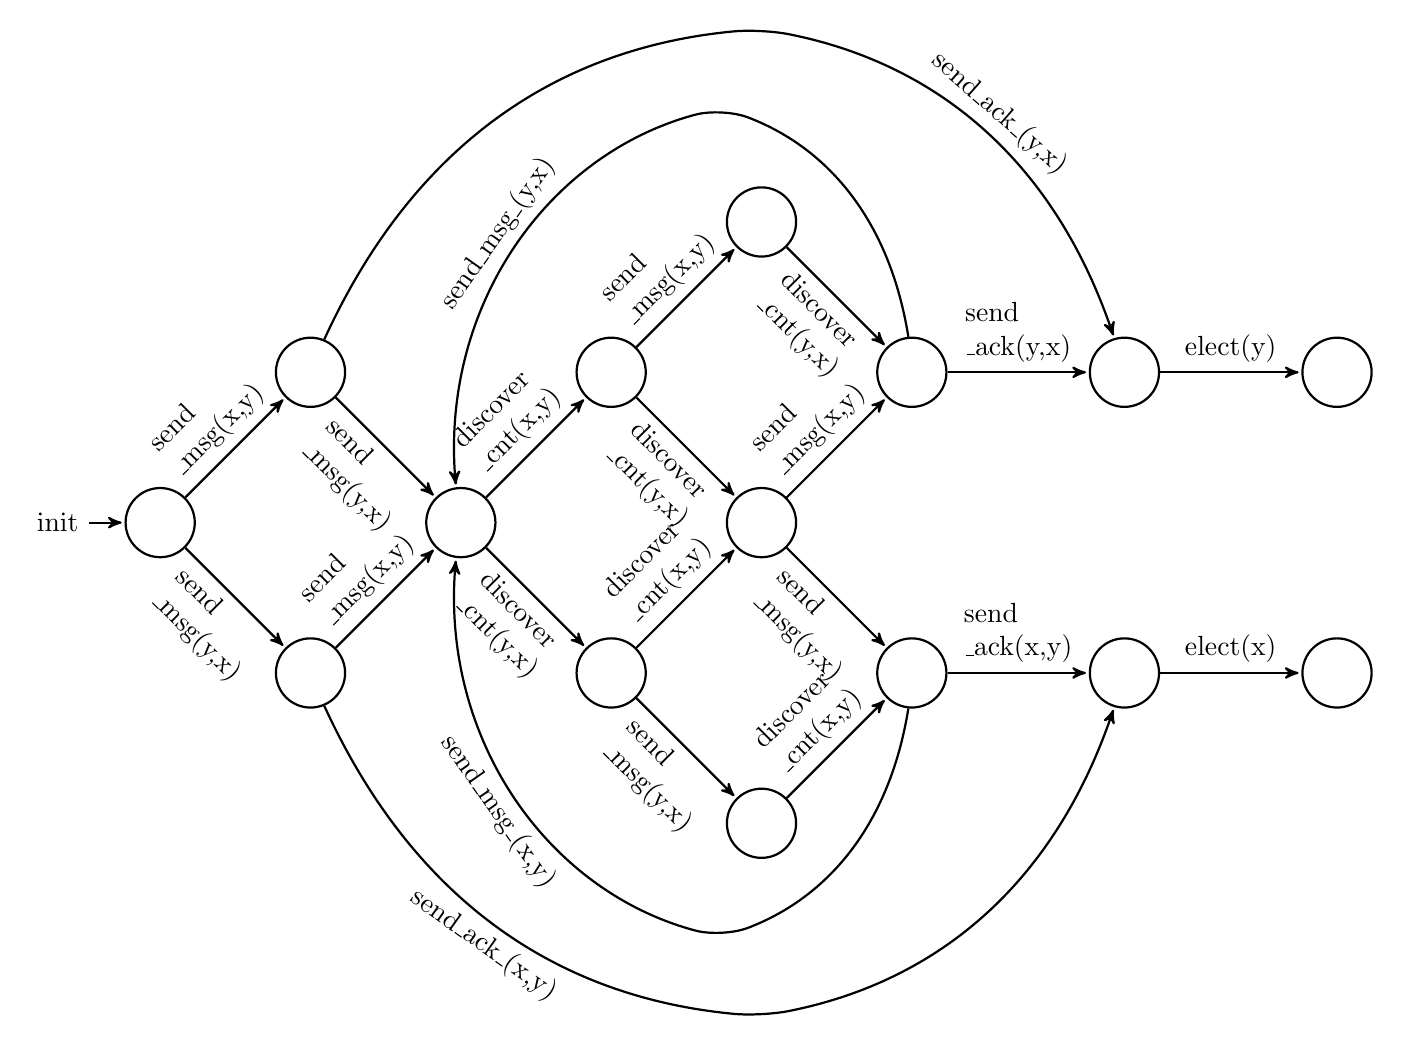
\begin{tikzpicture}[->,>=stealth',shorten >=1pt,auto,node distance=2.7cm,
                    thick, el/.style = {align=left, sloped}]
  \tikzstyle{every state}=[]

  \node[initial,initial text=init,state] (init)  {};
  \node[state,align=center] (x_send)            [above right of=init] {};
  \node[state,align=center] (y_send)            [below right of=init] {};
  \node[state,align=center] (cnt)               [below right of=x_send] {};
  \node[state,align=center] (delay_x)           [above right of=cnt] {};
  \node[state,align=center] (delay_y)           [below right of=cnt] {};
  \node[state,align=center] (x_send_y)          [above right of=delay_x] {};
  \node[state,align=center] (y_send_x)          [below right of=delay_y] {};
  \node[state,align=center] (delay_x_y)         [below right of=delay_x] {};
  \node[state,align=center] (x_send_y_delay)    [below right of=x_send_y] {};
  \node[state,align=center] (y_send_x_delay)    [above right of=y_send_x] {};
  \node[state,align=center] (y_ack)             [right of=x_send_y_delay]{};
  \node[state,align=center] (x_ack)             [right of=y_send_x_delay]{};
  \node[state,align=center] (y_leader)          [right of=y_ack]{};
  \node[state,align=center] (x_leader)          [right of=x_ack]{};
  
  \coordinate[shift={(-0.5cm,1cm)}] (interm1) at (x_send_y.north);
  \coordinate[shift={(-0.5cm,-1cm)}] (interm2) at (y_send_x.south);
  \coordinate[shift={(0cm, 2cm)}] (interm3) at (x_send_y.north);
  \coordinate[shift={(0cm, -2cm)}] (interm4) at (y_send_x.south);
  
  \path (init)      edge node[el,above] {send\\\_msg(x,y)}      (x_send)
                    edge node[el,below] {send\\\_msg(y,x)}      (y_send)
        (x_send)    edge node[el,below] {send\\\_msg(y,x)}      (cnt)
        (y_send)    edge node[el,above] {send\\\_msg(x,y)}      (cnt)
        (cnt)       edge node[el,above] {discover\\\_cnt(x,y)}  (delay_x)
                    edge node[el,below] {discover\\\_cnt(y,x)}  (delay_y)
        (delay_x)   edge node[el,above] {send\\\_msg(x,y)}      (x_send_y)
                    edge node[el,below] {discover\\\_cnt(y,x)}  (delay_x_y)
        (delay_y)   edge node[el,below] {send\\\_msg(y,x)}      (y_send_x)
                    edge node[el,above] {discover\\\_cnt(x,y)}  (delay_x_y)
        (delay_x_y) edge node[el,above] {send\\\_msg(x,y)}      (x_send_y_delay)
                    edge node[el,below] {send\\\_msg(y,x)}      (y_send_x_delay)
        (x_send_y)  edge node[el,below] {discover\\\_cnt(y,x)}  (x_send_y_delay)
        (y_send_x)  edge node[el,above] {discover\\\_cnt(x,y)}  (y_send_x_delay)
        (y_send_x_delay) edge node[el,above] {send\\\_ack(x,y)} (x_ack)
        (x_send_y_delay) edge node[el,above] {send\\\_ack(y,x)} (y_ack)
        (y_ack)     edge node[el,above] {elect(y)}                  (y_leader)
        (x_ack)     edge node[el,above] {elect(x)}                  (x_leader)
        ;
        
    \draw[rounded corners=10pt] (y_send_x_delay) to[bend left] (interm2) to[bend left=40] node[el,below] {send\_msg\_(x,y)} (cnt);
    \draw[rounded corners=10pt] (x_send_y_delay) to[bend right] (interm1) to[bend right=40] node[el,above] {send\_msg\_(y,x)} (cnt);
    \draw[rounded corners=10pt] (x_send) to[bend left] (interm3) to[bend left] node[el,above] {send\_ack\_(y,x)} (y_ack);
    \draw[rounded corners=10pt] (y_send) to[bend right] node[el,below] {send\_ack\_(x,y)} (interm4) to[bend right] (x_ack);
    
\end{tikzpicture}
    %}
    \caption{Automata for third refinment}
    \label{fig:my_label}
\end{figure}

\end{document}
